%!TEX root = main.tex

\section{Modeling approach}

Engineering correlations, reduced-order models, and CFD modeling techniques were used to investigate the effects of recycled gas on the operation of a fluidized-bed biomass pyrolysis reactor. The following sections discuss approaches implemented in this work for calculating gas properties and the associated effects on fluidization conditions and pyrolysis yields.

\subsection{Gas properties}

Density (kg/m$^3$) of an individual gas is calculated from the ideal gas law

\begin{equation}
    \rho_{gas} = \frac{P\;M}{R\;T}
\end{equation}

\noindent where P is pressure (Pa), M is molecular weight (g/mol), R is the gas constant [(m$^3$ Pa) / (K mol)], and T is temperature (K). Gas viscosity ($\mu$P) is given as

\begin{equation}
    \mu_{gas} = A + B\,T + C\,T^2 + D\,T^3
\end{equation}

\noindent where coefficients A, B, C, and D are obtained for a given gas from tables in Yaws' Handbook and T is gas temperature (K). Thermal conductivity (k) of the gas is given as

\begin{equation}
    k_{gas} = A + B\,T + C\,T^2 + D\,T^3
\end{equation}

\noindent where coefficients A, B, C, and D are also from the Yaws' Handbook and T is again the gas temperature (K).

For a gas mixture, density is calculated as a weighted average of the individual gas densities. The viscosity of a gas mixture can be calculated from a variety of correlations.

\subsection{Fluidization correlations}

Here.

\subsection{CFD simulation}

Here.

\subsection{Pyrolysis kinetics}

The Di Blasi kinetic scheme was implemented to predict the conversion of the biomass into gas, tar, and char products. Figure \ref{fig:blasi} gives an overview of the Di Blasi scheme and its reaction mechanisms. Reactions 1--3 are the primary conversion of the biomass while reactions 4--5 are secondary reactions that reduce tar yield at long residence times.

\begin{figure}[H]
    \centering
    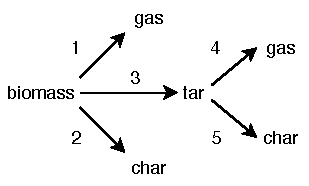
\includegraphics[width=0.35\textwidth]{blasi.pdf}
    \caption{Diagram of the Di Blasi pyrolysis kinetics for conversion of biomass to gas, tar, and char products.}
    \label{fig:blasi}
\end{figure}

\begin{table}[H]
    \centering
    \caption{Kinetic parameters for the Di Blasi biomass pyrolysis scheme.}
    \begin{tabular}{crrr}
        \hline
        Reaction    & A (1/s)               & E (kJ/mol)    & Reference     \\
        \hline
        1           & $1.3 \times 10^8$     & 140           & ??            \\
        2           & $2.0 \times 10^8$     & 133           & ??            \\
        3           & $1.08 \times 10^7$    & 121           & ??            \\
        4           & $4.28 \times 10^6$    & 108           & ??            \\
        5           & $1.0 \times 10^6$     & 108           & ??            \\
        \hline
    \end{tabular}
\end{table}

\subsection{Parameters}

Parameters for the reduced-order model and CFD simulations are provided in Table \ref{tab:params}. Biomass particle characteristics and properties are representative of loblolly pine. Bed particle characteristics are for typical sand material. Operating conditions and reactor dimensions are based on the previously discussed NREL 2FBR fluidized bed pyrolysis unit.

\begin{table}[H]
    \centering
    \caption{Biomass, bed, and reactor modeling parameters. Particle diameters represent the Sauter-mean diameter.}
    \begin{tabular}{lrll}
        \hline
        Parameter & Value & Units & Description \\
        \hline
        d$_\textrm{p,\,bed}$            & 235   & \textmugreek m & diameter of bed Particle      \\
        \straightphi$_\textrm{bed}$     & 0.0   &                & sphericity of bed particle    \\
        d$_\textrm{p,\,bio}$            & 135   & \textmugreek m & diameter of biomass particle  \\
        \straightphi$_\textrm{bio}$     & 0.0   &                & sphericity of biomass particle\\
        \textrho$_\textrm{bio}$         & 540   & kg/m$^3$       & density of biomass particle   \\
        h$_\textrm{reactor}$            & 43.18 & cm             & reactor height                \\
        h$_\textrm{static}$             & 10.16 & cm             & static bed height             \\
        T                               & 773   & K              & reactor temperature           \\
        \hline
    \end{tabular}
    \label{tab:params}
\end{table}
